% !TeX spellcheck =  en_GB, sp_SP

\newglossaryentry{minimum}
{
	name=mínimo,
	description={Dado un conjunto de números reales, el mínimo\index{mínimo} es el menor de esos números.},
	first={mínimo},text={mínimo}
}


\newglossaryentry{maximum}
{name=máximo,
 %description={Given a set of real numbers, the maximum\index{maximum} is the largest of those numbers.},
     description={El máximo\index{máximo} de un conjunto $\mathcal{A} \subseteq \mathbb{R}$ 
	 de números reales es el elemento más grande en ese conjunto, si tal elemento existe. Un conjunto $\mathcal{A}$ 
	 tiene un máximo si está acotado superiormente y alcanza su \gls{supremum} \cite[Sec.~1.4]{RudinBookPrinciplesMatheAnalysis}.},
 first={máximo},text={máximo}
}

\newglossaryentry{supremum}
{name=supremo (o mínimo de las cotas superiores),
	description={El supremo\index{supremo (o mínimo de las cotas superiores)} de un conjunto de números reales es 
		el número más pequeño que es mayor o igual que todos los elementos del conjunto. Formalmente, un número real 
		$a$ es el supremo de un conjunto $\mathcal{A} \subseteq \mathbb{R}$ si: 1) $a$ 
		es una cota superior de $\mathcal{A}$; y 2) ningún número menor que $a$ es una cota superior de $\mathcal{A}$. 
		Todo conjunto no vacío de números reales que esté acotado superiormente tiene un supremo,aun si no contiene su supremo como un elemento \cite[Sec.~1.4]{RudinBookPrinciplesMatheAnalysis}.},
	first={supremo (o mínimo de las cotas superiores)},text={supremo}
}

\newglossaryentry{discrepancy}
{name=discrepancia,
	description={
		Considere\index{discrepancia} una aplicacion de  \gls{fl} con \gls{netdata} 
		representada por un \gls{empgraph}. Los métodos de \gls{fl} utilizan una medida de discrepancia para  
		comparar los mapas  de \gls{hypothesis} generados por los  \gls{localmodel}s en los nodos $\nodeidx,\nodeidx'$ 
		conectados por una arista en el \gls{empgraph}.},
	first={discrepancia},text={discrepancia}
}



\newglossaryentry{hfl}
{name={aprendizaje federado horizontal (horizontal FL)},
	description={
		El aprendizaje federado horizontal\index{aprendizaje federado horizontal (horizontal FL)} utiliza \gls{localdataset}s constituidos por diferentes
		\gls{datapoint}s, pero emplea las mismas \gls{feature}s para caracterizarlos \cite{HFLChapter2020}.
		Por ejemplo, la predicción meteorológica utiliza una red de estaciones meteorológicas
		(observación) distribuidas espacialmente. Cada estación mide las mismas cantidades, como
		la temperatura diaria, la presión atmosférica y la precipitación. Sin embargo,
		distintas estaciones miden las características o \gls{feature}s de diferentes regiones espaciotemporales.
		Cada región espaciotemporal representa un \gls{datapoint} individual, caracterizado por las mismas \gls{feature}s
		(por ejemplo, temperatura diaria o presión atmosférica).
	},
	first={aprendizaje federado horizontal},text={horizontal FL}
}

\newglossaryentry{dimred}
{name={reducción de dimensionalidad},
	description={
		Los métodos de reducción de dimensionalidad\index{reducción de dimensionalidad}
		mapean (normalmente muchos) \gls{feature}s originales a un conjunto (relativamente pequeño) de
		nuevos \gls{feature}s. Estos métodos pueden utilizarse para visualizar \gls{datapoint}s
		aprendiendo dos \gls{feature}s que sirvan como coordenadas de una representación
		en un \gls{scatterplot}.
	},
	first={reducción de dimensionalidad},text={reducción de dimensionalidad}
}



\newglossaryentry{ml}
{name={aprendizaje automático (ML)},
	description={
		El aprendizaje automático\index{aprendizaje automático (ML)} tiene como objetivo predecir
		una \gls{label} a partir de las \gls{feature}s de un \gls{datapoint}. Los métodos de ML logran esto
		aprendiendo una \gls{hypothesis} de un \gls{hypospace} (o \gls{model})
		mediante la minimización de una \gls{lossfunc} \cite{MLBasics,HastieWainwrightBook}.
		Una formulación precisa de este principio es el \gls{erm}.
		Diferentes métodos de ML se obtienen de distintas elecciones de diseño para los
		\gls{datapoint}s (sus \gls{feature}s y \gls{label}),
		el \gls{model}, y la \gls{lossfunc} \cite[Cap. 3]{MLBasics}.
	},
	first={aprendizaje automático},text={ML}
}


\newglossaryentry{featlearn}
{name={aprendizaje de características},
	description={Consideremos una aplicación de \gls{ml} con \gls{datapoint}s caracterizados por 
	\gls{feature}s crudas $\featurevec \in \featurespace$. El aprendizaje de características\index{aprendizaje de características}
	se refiere a la tarea de aprender un mapeo
		$$\featuremapvec: \featurespace \rightarrow \featurespace': \featurevec \mapsto \featurevec',$$ 
		que recibe como entrada las \gls{feature}s crudas $\featurevec \in \featurespace$ de un \gls{datapoint} y entrega nuevas
		\gls{feature}s $\featurevec' \in \featurespace'$ de un nuevo \gls{featurespace} $\featurespace'$. 
		Se obtienen diferentes métodos de aprendizaje de características a partir de diferentes elecciones de 
		$\featurespace,\featurespace'$, de un \gls{hypospace} $\hypospace$ de posibles mapeos $\featuremapvec$, 
		y de una medida cuantitativa de la utilidad de un mapeo específico $\featuremapvec \in \hypospace$. Por ejemplo, \gls{pca} utiliza $\featurespace \defeq \mathbb{R}^{\dimlocalmodel}$, $\featurespace' \defeq \mathbb{R}^{\dimlocalmodel'}$
		con $\dimlocalmodel' < \dimlocalmodel$, y un \gls{hypospace}
		$$\hypospace\defeq \big\{ \featuremapvec: \mathbb{R}^{\dimlocalmodel}
		\!\rightarrow\! \mathbb{R}^{\dimlocalmodel'}\!:\!\featurevec'\!\defeq\!\mF \featurevec \mbox{ con alguna } \mF \!\in\! \mathbb{R}^{\dimlocalmodel' \times \dimlocalmodel} \big\}.$$ \Gls{pca} mide la utilidad de un mapeo específico $\featuremapvec(\featurevec)= \mF \featurevec$ 
		por el \gls{minimum} error de reconstrucción lineal incurrido sobre un \gls{dataset}, 
$$ \min_{\mG \in \mathbb{R}^{\dimlocalmodel \times \dimlocalmodel'}} \sum_{\sampleidx=1}^{\samplesize} \normgeneric{\mG \mF \featurevec^{(\sampleidx)} - \featurevec^{(\sampleidx)}}{2}^{2}.$$ }, 
	first={aprendizaje de características},text={aprendizaje de características}
} 

\newglossaryentry{autoencoder}
{name={autoencoder},
	description={Un autoencoder\index{autoencoder} es un método de \gls{ml} que aprende simultáneamente un mapeo codificador
		$\hypothesis(\cdot) \in \hypospace$ y un mapeo decodificador $\hypothesis^{*}(\cdot) \in \hypospace^{*}$. 
		Es una instancia de \gls{erm} que utiliza una \gls{loss} calculada a partir del error de reconstrucción 
		$\featurevec - \hypothesis^{*}\big(  \hypothesis \big( \featurevec \big) \big)$.},
	first={autoencoder},text={autoencoder}
} 

\newglossaryentry{vfl}
{name={aprendizaje federado vertical (FL vertical)},description=
	{El aprendizaje federado vertical\index{aprendizaje federado vertical (FL vertical)} utiliza \gls{localdataset}s
	 formados por los mismos \gls{datapoint}s, pero caracterizados mediante diferentes \gls{feature}s \cite{VFLChapter}. 
    Por ejemplo, diferentes proveedores de salud podrían contener información
	 sobre la misma población de pacientes. Sin embargo, diferentes proveedores de salud
	 recopilan distintas mediciones (por ejemplo, valores sanguíneos, electrocardiogramas, radiografías de tórax)
	 para los mismos pacientes.},
	first={aprendizaje federado vertical (FL vertical)},text={FL vertical}
} 

\newglossaryentry{interpretability}
{name={interpretabilidad},description=
		{Un método de \gls{ml} es interpretable \index{interpretabilidad} por un usuario específico si
		puede anticipar adecuadamente las \gls{prediction}es entregadas por el método. 
		La noción de interpretabilidad puede precisarse utilizando medidas cuantitativas
		de la incertidumbre sobre las \gls{prediction}es \cite{JunXML2020}.},
		first={interpretabilidad},text={interpretabilidad}
}

\newglossaryentry{multitask learning}
{name={aprendizaje multitarea},description=
	{El aprendizaje multitarea\index{aprendizaje multitarea} tiene como objetivo aprovechar las relaciones entre diferentes \gls{learningtask}s. 
	Considere dos \gls{learningtask}s obtenidas del mismo \gls{dataset} de capturas de webcam.
	La primera tarea consiste en predecir la presencia de un ser humano, 
	mientras que la segunda consiste en predecir la presencia de un automóvil. Podría ser útil utilizar la misma estructura de \gls{deepnet} para ambas tareas y permitir que solo los \gls{weights} 
	de la capa de salida final sean diferentes.},
	first={aprendizaje multitarea},text={aprendizaje multitarea}
}

\newglossaryentry{learningtask}
{name={tarea de aprendizaje},description=
	{Consideremos\index{tarea de aprendizaje} un \gls{dataset} $\dataset$ constituido por varios \gls{datapoint}s, cada uno 
	caracterizado por \gls{feature}s $\featurevec$. Por ejemplo, el \gls{dataset} $\dataset$ 
	podría estar constituido por imágenes de una base de datos particular. A veces puede ser útil 
	 representar un \gls{dataset} $\dataset$, junto con la elección de \gls{feature}s, por un \gls{probdist} $p(\featurevec)$. 
	 Una tarea de aprendizaje asociada a $\dataset$ consiste en una elección específica de la 
	 \gls{label} de un \gls{datapoint} y el correspondiente \gls{labelspace}. 
	 Dada una elección de la \gls{lossfunc} y el \gls{model}, una tarea de aprendizaje da lugar 
	 a una instancia de \gls{erm}. Así, también podríamos definir una tarea de aprendizaje mediante una instancia de \gls{erm}, es decir, 
	 mediante una \gls{objfunc}. Nótese que, para el mismo \gls{dataset}, obtenemos diferentes tareas de aprendizaje utilizando 
	 distintas elecciones de \gls{feature}s y \gls{label} de un \gls{datapoint}. Estas tareas de aprendizaje  
	 están relacionadas, ya que se basan en el mismo \gls{dataset}, y resolverlas conjuntamente 
	 (usando métodos de \gls{multitask learning}) es preferible a resolverlas de forma independiente \cite{Caruana:1997wk}, \cite{JungGaphLassoSPL}, \cite{CSGraphSelJournal}.
	 },
	first={tarea de aprendizaje},text={tarea de aprendizaje
}

\newglossaryentry{explainability}
{name={explicabilidad},
	description={
		Definimos\index{explicabilidad} la (subjetiva) explicabilidad de un método de \gls{ml}
		como el nivel de simulabilidad \cite{Colin:2022aa} de las \gls{prediction}es
		entregadas por un sistema de \gls{ml} a un usuario humano.
		Se pueden construir medidas cuantitativas para la explicabilidad (subjetiva) de un \gls{model} entrenado
		comparando sus \gls{prediction}es con las \gls{prediction}es proporcionadas por un usuario
		en un \gls{testset} \cite{Zhang:2024aa,Colin:2022aa}.
		Alternativamente, podemos usar \gls{probmodel}s para los \gls{data}
		y medir la explicabilidad de un \gls{model} de \gls{ml} entrenado mediante la entropía condicional
		(diferencial) de sus \gls{prediction}es, dadas las \gls{prediction}es del usuario \cite{JunXML2020,Chen2018}.
	},
	first={explicabilidad},text={explicabilidad}
}
	
\newglossaryentry{lime}
{name={Explicaciones Locales Interpretables e Independientes del Modelo (LIME)},description={
		Consideremos\index{Explicaciones Locales Interpretables e Independientes del Modelo (LIME)} 
		un \gls{model} entrenado (o una \gls{hypothesis aprendida}) $\widehat{\hypothesis} \in \hypospace$, 
		que asigna la \gls{featurevec} de un \gls{datapoint} a la \gls{prediction} $\widehat{\truelabel}= \widehat{\hypothesis}$. 
		Las explicaciones Locales Interpretables e Independientes del Modelo (LIME) son una tecnica para explicar 
		el comportamiento de $\widehat{\hypothesis}$, localmente, alrededor de un \gls{datapoint} con \gls{featurevec} $\featurevec^{(0)}$ \cite{Ribeiro2016}. 
		La explicación se da en forma de una aproximación local $g \in \hypospace'$ de $\widehat{\hypothesis}$ (véa Fig.\ \ref{fig_lime}). 
		Esta aproximación puede obtenerse mediante una instancia de \gls{erm} con un 
		\gls{trainset} diseñado cuidadosamente. En particular, el \gls{trainset} consiste en \gls{datapoint}s con 
		\gls{featurevec} $\featurevec$ cercana a $\featurevec^{(0)}$ y la (pseudo-)etiqueta $\widehat{\hypothesis}(\featurevec)$. 
		Nótese que podemos utilizar un \gls{model} $\hypospace'$ diferente para la aproximación que 
		el \gls{model} original $\hypospace$. Por ejemplo, podemos usar un \gls{decisiontree} 
		para aproximar (localmente) una \gls{deepnet}. Otra elección ampliamente utilizada para $\hypospace'$ es 
		el \gls{linmodel}. 
		\begin{figure}[htbp]
		\begin{center}
		\begin{tikzpicture}
			\begin{axis}[
				axis lines=middle,
				xlabel={$\featurevec$},
				ylabel={$\truelabel$},
				xtick=\empty,
				ytick=\empty,
				xmin=0, xmax=6,
				ymin=0, ymax=6,
				domain=0:6,
				samples=100,
				width=10cm,
				height=6cm,
				clip=false
			]
			  % Non-linear model h(x)
 			\addplot[blue, thick, domain=0:6] {2 + sin(deg(x))} node[pos=0.85, above right,yshift=3pt] {$\widehat{\hypothesis}(\featurevec)$};
			 % Feature value x0
 			\addplot[dashed, gray] coordinates {(3,0) (3,6)};
			% Piecewise constant local approximation g(x)
 			\addplot[red, thick, domain=2.5:3.5] {2 + sin(deg(3))} node[pos=0.9, above] {$g(\featurevec)$};
			% Optional: mark the point of approximation
 			\addplot[mark=*] coordinates {(3, {2 + sin(deg(3))})};
			\node at (axis cs:3,-0.3) {$\featurevec^{(0)}$};
			\end{axis}
		  \end{tikzpicture}
		\end{center}
		\caption{Para explicar un \gls{model} $\widehat{\hypothesis} \in \hypospace$ entrenado, alrededor de un \gls{featurevec} $\featurevec^{(0)}$, podemos usar una aproximación local $g \in \hypospace'$. }
		\end{figure}\label{fig_lime}},
	first={LIME},text={LIME}
}



\newglossaryentry{linmodel}{name={modelo lineal},
	description={Consideremos\index{modelo lineal} \gls{datapoint}s, cada uno caracterizado por una \gls{featurevec} numérica
		$\featurevec \in \mathbb{R}^{\featuredim}$. Un  \gls{model} lineal es 
		un \gls{hypospace} que consiste en todos los mapeos lineales, 
	\begin{equation} 
		\label{equ_def_lin_model_hypspace_dict}
		\linmodel{\nrfeatures} \defeq \left\{ \hypothesis(\featurevec)= \weights^{T} \featurevec: \weights \in \mathbb{R}^{\nrfeatures} \right\}. 
	\end{equation} 
	Nótese que \eqref{equ_def_lin_model_hypspace_dict} define toda una familia de \gls{hypospace}s, parametrizada por el número
	 $\nrfeatures$ de \gls{feature}s que se combinan linealmente para formar la 
	\gls{prediction} $\hypothesis(\featurevec)$. La elección de diseño de $\nrfeatures$ se guía por \gls{compasp} 
	(por ejemplo, reducir $\nrfeatures$ implica menor computación), por \gls{statasp} (por ejemplo, aumentar $\nrfeatures$ podría 
	reducir el error de \gls{prediction}), y por la \gls{interpretability}. Un \gls{model} lineal que utiliza pocas 
	\gls{feature}s cuidadosamente elegidas suele considerarse más interpretable \cite{Ribeiro2016,rudin2019stop}.}, 
  first={modelo lineal},text={modelo lineal}}
	
	
\newglossaryentry{gradstep}{name={paso de gradiente},description={Dada una función diferenciable \gls{differentiable} 
		 de valores reales $f(\cdot): \mathbb{R}^{\nrfeatures} \rightarrow \mathbb{R}$ 
		 y un vector $\weights \in \mathbb{R}^{\nrfeatures}$, el paso de \gls{gradient} \index{gradient step} 
		 actualiza $\weights$ sumándole el negativo escalado del \gls{gradient} $\nabla f(\weights)$ para obtener 
		 el nuevo vector (véase la Figura \ref{fig_basic_GD_step_single_dict})
		 \begin{equation}
		 \label{equ_def_gd_basic_dict} 
		\widehat{\weights}  \defeq \weights - \lrate \nabla f(\weights).
		\end{equation} 
		Matemáticamente, el paso de \gls{gradient} es un operador (típicamente no lineal) $\mathcal{T}^{(f,\lrate)}$
		que está parametrizado por la función $f$ y el \gls{stepsize} $\lrate$. 
		\begin{figure}[H]
			\begin{center}
				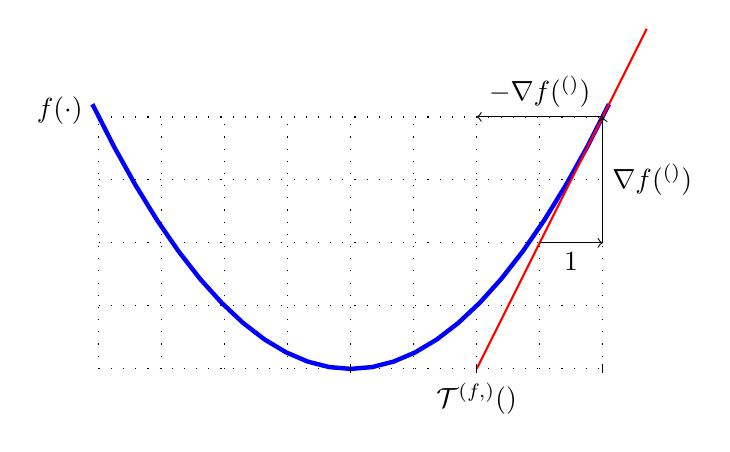
\begin{tikzpicture}[scale=0.8]
					\draw[loosely dotted] (-4,0) grid (4,4);
					\draw[blue, ultra thick, domain=-4.1:4.1] plot (\x,  {(1/4)*\x*\x});
					\draw[red, thick, domain=2:4.7] plot (\x,  {2*\x - 4});
					\draw[<-] (4,4) -- node[right] {$\nabla f(\weights^{(\itercntr)})$} (4,2);
					\draw[->] (4,4) -- node[above] {$-\lrate \nabla f(\weights^{(\itercntr)})$} (2,4);
					\draw[<-] (4,2) -- node[below] {$1$} (3,2) ;
					%\draw[->] (-4.25,0) -- (4.25,0) node[right] {$a$};
					\node[left] at (-4.1, 4.1) {$f(\cdot)$}; 
					\draw[shift={(0,0)}] (0pt,2pt) -- (0pt,-2pt) node[below] {$\overline{\weights}$};
					\draw[shift={(4,0)}] (0pt,2pt) -- (0pt,-2pt) node[below] {$\weights$};
					\draw[shift={(2,0)}] (0pt,2pt) -- (0pt,-2pt) node[below] {$\mathcal{T}^{(f,\lrate)}(\weights)$};
				\end{tikzpicture}
			\end{center}
			\caption{El paso básico de \gls{gradient} \eqref{equ_def_gd_basic_dict} mapea un vector $\weights$ 
			al vector actualizado $\weights'$. Define un operador 
			$\mathcal{T}^{(f,\lrate)}(\cdot): \mathbb{R}^{\nrfeatures} \rightarrow \mathbb{R}^{\nrfeatures}:
			 \weights \mapsto \widehat{\weights}$.}
			\label{fig_basic_GD_step_single_dict}
		\end{figure}
		Nótese que el paso de \gls{gradient} \eqref{equ_def_gd_basic_dict} optimiza localmente - 
		en una \gls{neighborhood} cuyo tamaño está determinado por el \gls{stepsize} $\lrate$ - una aproximación lineal 
		de la función $f(\cdot)$. Un  \gls{generalization} natural de \eqref{equ_def_gd_basic_dict} es optimizar localmente
		la función misma - en lugar de su aproximación lineal - de tal manera que:
		\begin{align} 
		\label{equ_approx_gd_step_dict}
		\widehat{\weights} = \argmin_{\weights' \in \mathbb{R}^{\dimlocalmodel}} f(\weights')\!+\!(1/\lrate)\normgeneric{\weights-\weights'}{2}^2. 
		\end{align}
		Intencionalmente usamos el mismo símbolo $\lrate$ para el parámetro en \eqref{equ_approx_gd_step_dict} 
		que en el \gls{stepsize} de \eqref{equ_def_gd_basic_dict}. Mientras mayor sea el valor de $\lrate$ en 
		\eqref{equ_approx_gd_step_dict}, más progreso hará la actualización en la reducción del valor de la función $f(\widehat{\weights})$. 
		Nótese que, al igual que el paso de \gls{gradient}  \eqref{equ_def_gd_basic_dict}, 
		la actualización \eqref{equ_approx_gd_step_dict} también define un operador (típicamente no lineal)  
		parametrizado por la función $f(\cdot)$ y el parámetro $\lrate$. Para una función \gls{convex}  
		$f(\cdot)$, este operador es conocido como el \gls{proxop} de $f(\cdot)$ \cite{ProximalMethods}. 
		},first={paso de gradiente},text={paso de gradiente}}
	

\newglossaryentry{proxop}{name={operador proximal},description={Dada una funcion\gls{convex}\index{operador proximal}   
		 $f(\weights')$, definimos su operador proximal como \cite{ProximalMethods,Bauschke:2017} 
		$$\proximityop{f(\cdot)}{\weights}{\rho}\defeq \argmin_{\weights' \in \mathbb{R}^{\dimlocalmodel}} \bigg[ f(\weights')\!+\!(\rho/2) \normgeneric{\weights- \weights'}{2}^{2}\bigg] \mbox{ with } \rho > 0. $$ 
		Como se ilustra en la Figura \ref{fig_proxoperator_opt_dict}, evaluar el operador proximal 
		equivale a minimizar una variante penalizada de $f(\weights')$. El término de penalización es 
		la distancia euclidiana cuadrada escalada hacia un vector dado $\weights$ (que es la entrada del operador proximal). 
		%\Gls{convex} functions for which the proximal operator can be computed efficiently 
		%is sometimes referred to as \emph{proximable} or \emph{simple} \cite{Condat2013}. 
		El operador proximal puede interpretarse como una \gls{generalization} del \gls{gradstep}, definido 
		para una función \gls{smooth} y \gls{convex} $f(\weights')$. De hecho, realizar un 
		\gls{gradstep} con \gls{stepsize} $\lrate$ en el vector actual $\weights$ 
		es lo mismo que aplicar el \gls{proxop}de la función $\tilde{f}(\weights')= \big( \nabla f(\weights)\big)^{T} (\weights'-\weights)$ 
		y usar $\rho=1/\lrate$.
			\begin{figure}[H]
			\begin{center}
				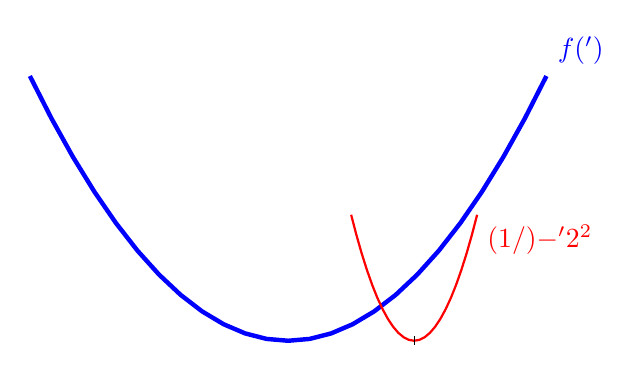
\begin{tikzpicture}[scale=0.8]
					% Original quadratic function
					\draw[blue, ultra thick, domain=-4.1:4.1] plot (\x, {(1/4)*\x*\x}) node[above right] {$f(\weights')$};		
					% Quadratic function with larger curvature, centered at w = 2
					\draw[red, thick, domain=1:3] plot (\x, {2*(\x - 2)*(\x - 2)}) node[below right] {$(1/\lrate)\normgeneric{\weights-\weights'}{2}^{2}$};
					% Axes
					% Minimum point of second curve
					\draw[shift={(2,0)}] (0pt,2pt) -- (0pt,-2pt) node[below] {$\weights$};
					%\node at (2,0.5) [anchor=north] {$\weights$};
				\end{tikzpicture}
			\end{center}
			\caption{Un \gls{gradstep} generalizado actualiza un vector $\weights$ minimizando una versión penalizada 
				de la función $f(\cdot)$. El término de penalización es la distancia euclidiana cuadrada escalada entre 
				la variable de optimización $\weights'$ y el vector dado $\weights$.\label{fig_proxoperator_opt_dict}}
		\end{figure}
		},first={operador proximal},text={operador proximal}}

\newglossaryentry{proximable}{name={proximable},description={Una funcion \index{proximable} 
		\gls{convex} para la cual el \gls{proxop} puede calcularse de manera eficiente 
		se denomina a veces proximable o simple \cite{Condat2013}.},
		first={proximable},text={proximable}
		
		}


\newglossaryentry{connected}
		{name={grafo conexo},
			description={
				Un \gls{graph} no dirigido\index{grafo conexo} $\graph=\pair{\nodes}{\edges}$ es conexo si todo subconjunto no vacío $\nodes' \subset \nodes$
				tiene al menos una arista que lo conecta con $\nodes \setminus \nodes'$.
			},
			first={grafo conexo},text={grafo conexo}
		}
	
	

\newglossaryentry{mvndist}{name ={distribución normal multivariante},description=
{
	La distribución normal multivariante\index{distribución normal multivariante} $\mvnormal{\vm}{\mC}$ es una
	familia importante de \gls{probdist}s para una \gls{rv} continua $\featurevec \in \mathbb{R}^{\nrfeatures}$ \cite{BertsekasProb,GrayProbBook,Lapidoth09}.
	Esta familia está parametrizada por la \gls{mean} $\vm$ y la \gls{covmtx} $\mC$ de $\featurevec$.
	Si la \gls{covmtx} es invertible, la \gls{probdist} de $\featurevec$ es
	$$p(\featurevec) \propto \exp\bigg(-(1/2) \big( \featurevec - \vm \big)^{T} \mC^{-1} \big( \featurevec - \vm \big) \bigg).$$
},
first={distribución normal multivariante},text={distribución normal multivariante}
}

\newglossaryentry{statasp}{name ={aspectos estadísticos}, description={Por aspectos estadísticos\index{aspectos estadísticos} 
		de un método de \gls{ml},  nos referimos a las propiedades de la \gls{probdist} de su salida bajo 
		un \gls{probmodel} para los \gls{data} introducidos en el método.},first={aspectos estadísticos},text={aspectos estadísticos}}

\newglossaryentry{compasp}{name ={aspectos computacionales}, description={Por aspectos 
		computacionales\index{aspectos computacionales} de un método de \gls{ml}, nos referimos principalmente a los recursos 
		computacionales requeridos para su implementación.
		Por ejemplo, si un método de \gls{ml} utiliza técnicas 
		de optimización iterativas para resolver \gls{erm}, sus aspectos computacionales incluyen: 1) cuántas 
		many operaciones aritméticas se necesitan para implementar una sola iteración(\gls{gradstep}); 
		y 2) cuántas iteraciones se requieren para obtener \gls{modelparams} útiles. Un ejemplo 
		importante de técnica de optimización iterativa es el  \gls{gd}.}, first={aspectos computacionales},text={aspectos computacionales}}

\newglossaryentry{zerooneloss}{name={$\bf 0/1$ loss},
	description={La \gls{loss} $0/1$ \index{$0/1$ loss} $\lossfunczo{\pair{\featurevec}{\truelabel}}{\hypothesis}$ 
		mide la calidad de un \gls{classifier} $\hypothesis(\featurevec)$ que genera una 
		\gls{prediction} $\predictedlabel$ (por ejemplo, mediante un umbral como en \eqref{equ_def_threshold_bin_classifier_dict}) 
		para la \gls{label} $\truelabel$ de un \gls{datapoint} con \gls{feature}s $\featurevec$. Es igual a $0$ si 
		la \gls{prediction} es correcta, es decir, 
	$\lossfunczo{\pair{\featurevec}{\truelabel}}{\hypothesis}=0$ cuando $\predictedlabel=\truelabel$. Es igual 
	a $1$ si la \gls{prediction} es incorrecta, es decir, $\lossfunczo{\pair{\featurevec}{\truelabel}}{\hypothesis}=1$ 
	cuando $\predictedlabel\neq\truelabel$.},
	sort=zerooneloss, 
   first={$0/1$ loss},text={$0/1$ loss}}

\newglossaryentry{probability}{name={probabilidad},
	description={Asignamos \index{probabilidad} un valor de probabilidad, típicamente elegido en el 
		intervalo $[0,1]$, a cada evento que pueda ocurrir en un experimento aleatorio \cite{KallenbergBook,BertsekasProb,BillingsleyProbMeasure,HalmosMeasure}.},
		first={probabilidad},text={probabilidad}}
	
\newglossaryentry{underfitting}{name={subajuste},
	description={Consideremos\index{subajuste} un método de \gls{ml} que utiliza \gls{erm} para aprender una \gls{hypothesis}
	con el \gls{minimum} \gls{emprisk} en un \gls{trainset} dado.
	Dicho método presenta subajuste del \gls{trainset} si no es capaz de aprender una \gls{hypothesis}
	con un \gls{emprisk} suficientemente pequeño sobre el \gls{trainset}.
	Si un método sufre de subajuste, típicamente tampoco podrá aprender una \gls{hypothesis}
	con un \gls{risk} pequeño.},
	first={subajuste},text={subajuste}
		}

\newglossaryentry{overfitting}{name={sobreajuste},description={Consideremos\index{overfitting} un 
		método de \gls{ml} que utiliza \gls{erm} para aprender una \gls{hypothesis} con el \gls{minimum} \gls{emprisk} en 
		un \gls{trainset} dado. Dicho método presenta sobreajuste del \gls{trainset} si aprende 
		una \gls{hypothesis} con un \gls{emprisk} pequeño sobre el \gls{trainset} pero una \gls{loss} significativamente mayor fuera de él \gls{trainset}.},first={sobreajuste},text={sobreajuste}}

\newglossaryentry{gdpr}{name={reglamento general de protección de datos (RGPD)},description={
			El\index{reglamento general de protección de datos (RGPD)} RGPD
			fue promulgado por la Union Europea (EU), y entró en efecto el 25 de Mayo de 2018 \cite{GDPR2016}. 
			Protege la privacidad y los derechos sobre los \gls{data} de los individuos dentro de la EU. 
			El RGPD tiene implicaciones significativas sobre cómo se recopilan, almacenan y utilizan los \gls{data} en aplicaciones de \gls{ml}.
			Las disposiciones clave incluyen:
			\begin{itemize}
				\item \Gls{dataminprinc}: los sistemas de \gls{ml} deben utilizar únicamente la cantidad necesaria de  
				\gls{data} personal para su propósito.
				\item \Gls{transparency} y \gls{explainability}: los sistemas de \gls{ml} deben permitir a sus usuarios comprender 
				cómo se toman las decisiones que los afectan.
				\item Derechos del titular de los datos \Gls{data}:los usuarios deben tener la posibilidad de acceder, rectificar y eliminar sus \gls{data}, así como oponerse a decisiones automatizadas y perfiles.
				\item Responsabilidad: las organizaciones deben garantizar una seguridad robusta de los \gls{data} y demostrar 
				cumplimiento mediante documentación y auditorías periódicas.
			\end{itemize}
			}, 
	first={reglamento general de protección de datos (RGPD)},text={RGPD}}
	
\newglossaryentry{gaussrv}{name={variable aleatoria gaussiana (VA gaussiana)},description={
		Una \index{variable aleatoria gaussiana (VA gaussiana)} \gls{rv} gaussiana estándar es una \gls{rv} 
		real $x$ con \gls{pdf} \cite{papoulis,BertsekasProb,GrayProbBook}
		\begin{equation}
			\nonumber
			p(x) = \frac{1}{\sqrt{2\pi}} \exp^{-x^2/2}. 
		\end{equation}
		Dada una \gls{rv} gaussiana estándar $x$, podemos construir una \gls{rv} gaussiana general $x'$ con 
		\gls{mean} $\mu$ y \gls{variance} $\sigma^2$ mediante $x' \defeq \sigma (x+\mu)$. La \gls{probdist} de una 
		\gls{rv} gaussiana se conoce como distribución normal, denotada $\mathcal{N}(\mu,\sigma)$.  \\ 
		Un vector aleatorio gaussiano $\featurevec \in \mathbb{R}^{\featuredim}$ con 
		\gls{covmtx} $\mathbf{C}$ y \gls{mean} ${\bm \mu}$ puede construirse como 
		$\featurevec \defeq \mathbf{A} \big( \vz + {\bm \mu} \big)$. Aquí, $\mA$ 
		es cualquier matriz que satisface $\mA\mA^{T} = \mC$ y $\vz \defeq \big( z_{1},\ldots,z_{\featuredim} \big)^{T}$
		es un vector cuyos elementos son \gls{iid} gaussianas estándar \gls{rv}s $z_{1},\ldots,z_{\featuredim}$. Los procesos aleatorios gaussianos generalizan
		los vectores aleatorios gaussianos aplicando transformaciones lineales a 
		a secuencias infinitas de \gls{rv}s gaussianas estándar \cite{Rasmussen2006Gaussian}.\\
		Las \gls{rv}s gaussianas se utilizan ampliamente como \gls{probmodel}s en el análisis estadístico de métodos de \gls{ml}.
		Su importancia se debe, en parte, al teorema del límite central, que establece que el promedio de un número creciente de \gls{rv}s independientes
		(aunque no sean gaussianas) converge a una \gls{rv} gaussiana \cite{ross2013first}. 
},first={variable aleatoria gaussiana (VA gaussiana)},text={VA gaussiana}

\newglossaryentry{trustAI}{name={inteligencia artificial confiable (IA confiable)},description=
		{Además de los \gls{compasp} y los \gls{statasp}, un tercer aspecto principal 
		en el diseño de métodos de \gls{ml} es su confiabilidad\index{inteligencia artificial confiable (IA confiable)} \cite{pfau2024engineeringtrustworthyaideveloper}. 
		La Unión Europea ha propuesto siete requisitos clave (KRs) para una \gls{ai} confiable 
		(que típicamente se basa en métodos de \gls{ml}) \cite{ALTAIEU}: 
	\begin{enumerate}[label=\arabic*)]
		\item KR1 - Agencia y supervisión humana;
		\item KR2 - Robustez técnica y seguridad;
		\item KR3 - Privacidad y gobernanza de los \gls{data};
		\item KR4 - Transparencia;
		\item KR5 - Diversidad, no discriminación y equidad; 
		\item KR6 - Bienestar social y ambiental;
		\item KR7 - Responsabilidad. 
	\end{enumerate}
	},first={inteligencia artificial confiable (IA confiable)},text={trustworthy AI}}

\newglossaryentry{sqerrloss}{name={pérdida de error cuadrático},description={La \gls{loss} de
		error cuadrático\index{pérdida de error cuadrático} mide el error de \gls{prediction} de una 
		\gls{hypothesis} $\hypothesis$ al predecir una \gls{label} numérica $\truelabel \in \mathbb{R}$ 
		a partir de las \gls{feature}s $\featurevec$ de un \gls{datapoint}. Se define 
	como 
\begin{equation} 
	\nonumber
%	\label{equ_squared_loss_gls}
	\lossfunc{(\featurevec,\truelabel)}{\hypothesis} \defeq \big(\truelabel - \underbrace{\hypothesis(\featurevec)}_{=\predictedlabel} \big)^{2}. 
\end{equation} 
},first={pérdida de error cuadrático},text={pérdida de error cuadrático}}


\newglossaryentry{projection}{name={proyección}, 
      description={Consideremos\index{proyección} un subconjunto $\paramspace \subseteq \mathbb{R}^{\dimlocalmodel}$ del 
	   \gls{euclidspace} de dimensión $\dimlocalmodel$. Definimos la proyección $\projection{\paramspace}{\weights}$
	   de un vector $\weights \in \mathbb{R}^{\dimlocalmodel}$ sobre $\paramspace$ como
		\begin{equation} 
  	    \label{equ_def_proj_generic_dict}
 	     \projection{\paramspace}{\weights} = \argmin_{\weights' \in \paramspace} \normgeneric{\weights - \weights'}{2}. 
        \end{equation}
		 En otras palabras, $\projection{\paramspace}{\weights}$ es el vector en $\paramspace$ más cercano a $\weights$. 
		 La proyección está bien definida solo para aquellos subconjuntos $\paramspace$ para los cuales existe el \gls{minimum} anterior \cite{BoydConvexBook}.},
		 first={proyección},text={proyección}}


\newglossaryentry{projgd}{name={descenso por gradiente proyectado (GD proyectado)},
description={Consideremos un método basado en \gls{erm} que utiliza un \gls{model} parametrizado con  
un \gls{paramspace} $\paramspace \subseteq \mathbb{R}^{\dimlocalmodel}$. Aun si la
\gls{objfunc} de \gls{erm} es \gls{smooth}, no podemos usar el \gls{gd} básico, ya 
ya que este no toma en cuenta las restricciones sobre la variable de optimización (es decir, los \gls{modelparams}). 
El \gls{gd} proyectado\index{descenso por gradiente proyectado (GD proyectado)} 
extiende el \gls{gd} básico para controlar restricciones sobre la variable de optimización(es decir, los \gls{modelparams}). 
Una sola iteración del \gls{gd} proyectado consiste primero en realizar un \gls{gradstep} 
y luego proyectar el resultado sobre el \gls{paramspace}.
\begin{figure}[H]
	\begin{center}
		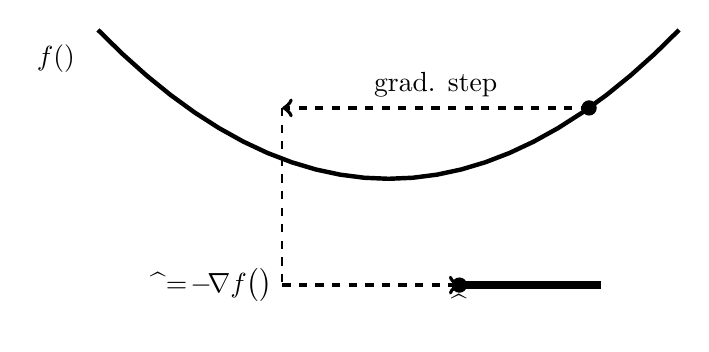
\begin{tikzpicture}[scale=0.9]
			\node [right] at (-5.1,1.7) {$f(\weights)$} ;
			\draw[ultra thick, domain=-4.1:4.1] plot (\x,  {(1/8)*\x*\x});
		%	\draw[dashed, thick, domain=1:3.6] plot (\x,  {\x - 1}) node[right] {$ f\big(\weights^{(\itercntr)}\big)\!+\!\big(\weights\!-\!\weights^{(\itercntr)}\big)^{T} \nabla f\big(\weights^{(\itercntr)}\big)$};
			\draw [fill] (2.83,1) circle [radius=0.1] node[right] {$\weights$};
			\draw[line width =0.5mm,dashed,->] (2.83,1) -- node[midway,above] {grad. step} (-1.5,1);
			\draw[line width =0.2mm,dashed] (-1.5,1) --(-1.5,-1.5)  node [below, left]{$\widehat{\weights}=\weights\!-\!\lrate \nabla f\big(\weights\big)$} ;
			\draw[line width =0.5mm,dashed,->] (-1.5,-1.5)  -- node[midway,above] {} (1,-1.5) ; 
			\draw [fill] (1,-1.5) circle [radius=0.1] node[below] {$\projection{\paramspace}{\widehat{\weights}}$};
			\draw[line width=1mm] (1,-1.5) -- (3,-1.5) node[midway, above] {$\paramspace$};
		\end{tikzpicture}
		\vspace*{-5mm}
	\end{center}
	\caption{\gls{gd} proyectado amplía un \gls{gradstep} básico con una \gls{projection} de regreso 
	al conjunto de restricciones $\paramspace$.}
	\label{fig_projected_GD_dict}
\end{figure}},first={descenso por gradiente proyectado (GD proyectado)},text={GD proyectado}}

\newglossaryentry{diffpriv}
{name=privacidad diferencial (DP),
 description={
 	Consideremos\index{differential privacy (DP)} un método de \gls{ml} $\algomap$ que recibe como entrada un \gls{dataset} (por ejemplo, el \gls{trainset} 
 	usado para \gls{erm}) y entrega una salida $\algomap(\dataset)$. La salida 
 	puede ser los \gls{modelparams} aprendidos o las \gls{prediction}es para ciertos \gls{datapoint}s. 
 	DP es una medida precisa de la \gls{privleakage} ocasionada al revelar dicha salida.
	Aproximadamente, un método de \gls{ml} es diferencialmente privado si la \gls{probdist} 
 	de la salida $\algomap(\dataset)$ no cambia significativamente cuando se modifica el \gls{sensattr} 
 	de un solo \gls{datapoint} del \gls{trainset}. Nótese que la DP 
 	se basa en un \gls{probmodel} para un método de \gls{ml}, es decir, interpretamos su salida $\algomap(\dataset)$ 
 	como la \gls{realization} de un \gls{rv}. La aleatoriedad en la salida puede asegurarse añadiendo intencionalmente la
 	\gls{realization} de una \gls{rv} auxiliar (ruido) a la salida del método de  \gls{ml}.
	}, 
	first = {privacidad diferencial (DP)}, text={DP} 
}

\newglossaryentry{privprot}
{name=protección de la privacidad,
    description={Consideremos\index{protección de la privacidad} un método de \gls{ml}  $\algomap$ que recibe como entrada 
	 una \gls{dataset} $\dataset$ y entega una salida $\algomap(\dataset)$. La salida 
	 puede ser los \gls{modelparams} aprendidos $\widehat{\weights}$ o una \gls{prediction} 
	 $\learnthypothesis(\featurevec)$ obtenida para un \gls{datapoint} específico con \gls{feature}s 
	 $\featurevec$. Muchas aplicaciones importantes de \gls{ml} involucran \gls{datapoint}s 
		que representan a personas. Cada \gls{datapoint} se caracteriza por \gls{feature}s $\featurevec$, 
		posiblemente una \gls{label} $\truelabel$, y un \gls{sensattr} $\sensattr$ (por ejemplo, un diagnóstico medico). 
		Mas o menos, la protección de la privacidad significa que debería ser imposible inferir, de la salida $\algomap(\dataset)$, 
		cualquier \gls{sensattr}s de los \gls{datapoint}s en $\dataset$. Matemáticamente, la protección de privacidad requiere que  
		el mapeo $\algomap(\dataset)$ no sea invertible. En general, el solo hacer que  $\algomap(\dataset)$ no sea invertible 
		no es suficiente. Necesitamos que sea suficientemente no invertible. 
	}, 
	first = {protección de la privacidad}, text={protección de la privacidad} 
}

\newglossaryentry{privleakage}
{
	name=filtración de privacidad,
	description={Consideremos\index{privacy leakage} una aplicacion de \gls{ml} que procesa un
	\gls{dataset} $\dataset$ y produce una salida, como las \gls{prediction}es 
	obtenidas para nuevos \gls{datapoint}s. Se produce una filtración de privacidad 
	cuando la salida contiene información privada sobre un \gls{feature} de un 
	\gls{datapoint} (que podría representar a una persona) en $\dataset$. Basado en la \gls{probmodel} 
	para la generacion de los \gls{data}, podemos medir la filtración de privacidad usando la \gls{mutualinformation} 
	entre la salida y la \gls{feature} sensible. Otra medida cuantitativa de la filtración de privacidad 
	es la \gls{diffpriv}. Las relaciones entre las diferentes medidas de filtración de privacidad han sido estudiadas en la literatura (véa \cite{InfThDiffPriv}). 
	}, 
	first = {filtración de privacidad}, text={filtración de privacidad} 
}



\newglossaryentry{probmodel}
{
	name=modelo probabilístico,
	description={Un \gls{model} probabilístico\index{modelo probabilístico} interpreta los \gls{datapoint}s 
		como \gls{realization}es de \gls{rv}s con una \gls{probdist} conjunta. Esta \gls{probdist} conjunta típicamente 
		incluye \gls{parameters} que deben seleccionarse manualmente or o aprenderse usando métodos de inferencia estadística  
		como la estimación por \gls{maxlikelihood} \cite{LC}. }, 
	first = {modelo probabilístico}, text={modelo probabilístico} 
}



\newglossaryentry{mean}
{
	name=media,
	description={La\index{media} \gls{expectation} $\expect \{ \featurevec \}$ de una \gls{rv} numérica $\featurevec$.}, 
		first = {media}, text={media} 
}

\newglossaryentry{variance}
{
	name={varianza},
	description={La\index{varianza} varianza de una \gls{rv} real $\feature$ se define como la \gls{expectation} 
		$\expect\big\{ \big( x - \expect\{x \} \big)^{2} \big\}$ de la diferencia cuadrada entre $\feature$ 
		y su \gls{expectation} $\expect\{x \}$. Extendemos esta definición a \gls{rv}s vectoriales$\featurevec$ 
		como $\expect\big\{ \big\| \featurevec - \expect\{\featurevec \} \big\|_{2}^{2} \big\}$.} ,
		first={varianza},text={varianza} 
}

\newglossaryentry{nn}
{
	name={vecino más cercano (NN)},
	description={Los métodos de vecino más cerano (NN)\index{vecino más cercano (NN)} aprenden una \gls{hypothesis} 
		$\hypothesis: \featurespace \rightarrow \labelspace$ cuyo valor $\hypothesis(\featurevec)$ 
		se determina únicamente por los \gls{neighbors} más cercanos dentro de un \gls{dataset}. Distintos 
		métodos usan diferentes medidas para determinar los \gls{neighbors} más cercanos. Si los \gls{datapoint}s 
		se caracterizan por \gls{featurevec}s numéricos, podemos usar la distancia euclidiana como medida.  
		the metric.},
	first={vecino más cercano (NN)},text={NN} 
}

\newglossaryentry{neighborhood}
{
	name={entorno},
	description={El\index{entorno} entorno de un nodo $\nodeidx \in \nodes$ es 
	el subconjunto de nodos constituido por los \gls{neighbors} de $\nodeidx$.},
	first={entorno},text={entorno} 
}


\newglossaryentry{neighbors}
{
	name={vecinos},
	description={Los\index{vecinos} vecinos de un nodo $\nodeidx \in \nodes$ 
	dentro de un \gls{empgraph} son los nodos $\nodeidx' \in \nodes \setminus \{ \nodeidx\}$ conectados con $\nodeidx$ por una arista.},
	first={vecinos},text={vecinos} 
}

\newglossaryentry{bias}
{
	name={sesgo},
	description={Consideremos\index{sesgo} un método de \gls{ml} que utiliza un \gls{hypospace} $\hypospace$ parametrizado. 
		Este aprende los \gls{modelparams} $\weights \in \mathbb{R}^{\dimlocalmodel}$ utilizando el \gls{dataset} $$ \dataset=\big\{ \pair{\featurevec^{(\sampleidx)}}{\truelabel^{(\sampleidx)}} \big\}_{\sampleidx=1}^{\samplesize}.$$ 
		Para analizar las propiedades del método de \gls{ml}, típicamente interpretamos los \gls{datapoint}s como \gls{realization}es 
		de \gls{iid} \gls{rv}s, $$ \truelabel^{(\sampleidx)} = \hypothesis^{(\overline{\weights})}\big( \featurevec^{(\sampleidx)} \big) + \bm{\varepsilon}^{(\sampleidx)}, \sampleidx=1,\ldots,\samplesize.$$ 
		Entonces podemos interpetar el método de \gls{ml} como un estimador $\widehat{\weights}$ 
		calculado a partir de $\dataset$ (por ejemplo, resolviendo \gls{erm}). El sesgo (cuadrado) del estimador $\widehat{\weights}$ 
		se define como $\biasterm^{2} \defeq \big\| \expect \{ \widehat{\weights}  \}- \overline{\weights}\big\|_{2}^{2}$. },
		first={sesgo},text={sesgo} 
}

\newglossaryentry{classification}
{name={clasificación},
description={La clasificación\index{classification} es la tarea de determinar una
	etiqueta $\truelabel$  con valor discreto para un \gls{datapoint}, basado únicamente en sus 
	 \gls(feature)s $\featurevec$. La etiqueta $\truelabel$ pertenece a un conjunto finito, como por ejemplo 
	$\truelabel \in \{-1,1\}$ o $\truelabel \in \{1,\ldots,19\}$, y representa la 
	categoría a la que pertenece el \gls{datapoint}.},
	first={clasificación},text={clasificación} 
}


% a bit awkward, come back to this. 
\newglossaryentry{privfunnel}
{name={embudo de privacidad},
description={El\index{privacy funnel} embudo de privacidad es un método para aprender \gls{feature}s 
	amigables con la privacidad de los \gls{datapoint}s \cite{PrivacyFunnel}.},
first={embudo de privacidad},text={embudo de privacidad} 
}




\newglossaryentry{condnr}
{
	name={número de condición},
	description={El número de condición\index{número de condición} $\kappa(\mathbf{Q}) \geq 1$ de una 
		matriz definida positiva $\mathbf{Q} \in \mathbb{R}^{\featurelen \times \featurelen}$ es el cociente 
		$\alpha /\beta  $ entre el 
		mayor $\alpha$ y el menor $\beta$ \gls{eigenvalue} de 
		$\mathbf{Q}$. El número de condición es útil para el análisis de métodos de \gls{ml}. 
		La complejidad computacional de los \gls{gdmethods} para \gls{linreg} depende críticamente del número 
		de condición de la matriz $\mQ = \mX \mX^{T}$, donde $\mX$  es la \gls{featuremtx}  
		del \gls{trainset}. Es por eso que desde una perspectiva computacional, preferimos \gls{feature}s de los 
		\gls{datapoint}s que hagan que $\mQ$ tenga un número de condición cercano a $1$.},first={número de condición},text={número de condición} 
}

\newglossaryentry{classifier}
{
	name={clasificador},
	description={Un clasificador\index{clasificador} es una \gls{hypothesis} (función) $\hypothesis(\featurevec)$ 
		usada para predecir una \gls{label} que toma valores de un \gls{labelspace} finito. Podemos usar directamente 
		el valor $\hypothesis(\featurevec)$ como \gls{prediction} $\predictedlabel$ para 
		la \gls{label}. pero normalmente se usa una función $\hypothesis(\cdot)$ que entrega 
		una cantidad numérica. La \gls{prediction} es obtenida a travez de un paso de umbral. 
		Por ejemplo, en un problema de \gls{classification} binaria con \label{labelspace} $\labelspace \in  \{ -1,1\}$, 
		podríamos usar una \gls{hypothesis} de valores reales $\hypothesis(\featurevec) \in \mathbb{R}$ 
		como clasificador. Una \gls{prediction} $\predictedlabel$ puede obtenerse mediante:  
		 \begin{equation} 
		 	\label{equ_def_threshold_bin_classifier_dict}
		 	\predictedlabel =1   \mbox{ for } \hypothesis(\featurevec)\!\geq\!0 \mbox{ and } 	\predictedlabel =-1  \mbox{ otherwise.}
	 		\end{equation}
		Podemos caracterizar un clasificador mediante sus \gls{decisionregion}es $\decreg{a}$, para 
		cada valor posible de \gls{label} $a \in \labelspace$. },first={clasificador},text={clasificador} 
}

\newglossaryentry{emprisk}
{name={riesgo empírico},
 description={El \gls{risk} empírico\index{riesgo empírico} $\emprisk{\hypothesis}{\dataset}$ 
 	de una \gls{hypothesis} sobre un \gls{dataset} $\dataset$ es la \gls{loss} promedio incurrida 
 	por $\hypothesis$ al aplicarse a los \gls{datapoint}s en el $\dataset$.},
 first={riesgo empírico},text={riesgo empírico} 
}

% is it not the number of edges connected to the node instead of the neigbors?  could be the same thing, just wondering about the actual definition here. 
\newglossaryentry{nodedegree}
{name={grado de nodo},
	description={El grado\index{grado de nodo} $\nodedegree{\nodeidx}$ de un nodo $\nodeidx \in \nodes$ 
		en un \gls{graph} no dirigido, es el número de sus \gls{neighbors}, es decir, $\nodedegree{\nodeidx} \defeq \big|\neighbourhood{\nodeidx}\big|$.},
		first={grado de nodo},text={grado de nodo} 
}

\newglossaryentry{graph}
{name={grafo},
	description={Un grafo\index{graph} $\graph = \pair{\nodes}{\edges}$ es un par compuesto por un  
		conjunto de nodos $\nodes$ y un conjunto de aristas $\edges$. En su forma màs general, un grafo se 
		específica por una función que asigna a cada arista $\edgeidx \in \edges$ un par de nodos \cite{RockNetworks}. 
		Un grupo importante de grafos son los grafos no dirigidos. Un grafo simple no dirigido  
		es obtenida identificando cada arista $\edgeidx \in \edges$ con dos nodos diferentes $\{\nodeidx,\nodeidx'\}$. 
		Los grafos etiquetados asignan un peso númerico especifico \gls{weights} $\edgeweight_{\edgeidx}$ a cada 
		arista $\edgeidx \in \edges$.},first={graph},text={graph} 
}

% i think UCB might be a unfinished definition. Check with Alex on this one. 

\newglossaryentry{ucb}
{name={límite superior de confianza (UCB)},
	description={Consideremos\index{límite superior de confianza (UCB)} una aplicacion de \gls{ml} 
		 que predice, en cada nueva iteración,
		 la acción óptima dentro de un conjunto finito de acciones posibles. Medimos la utilidad  
		 de una predicción \gls{prediction} (al tomar una accion específica) por un \gls{reward} númerico. 
		 Un \gls{probmodel} popular utilizado para este tipo de problema de decisiones secuenciales
		 es el problema multibrazo(multi-armed bandit) $\ldots$. 
		 
		 El premio obtenido por cada acción puede modelarse como una \gls{realization} de una\gls{rv} 
		 con cierta \gls{mean} y \gls{variance}.},first={límite superior de confianza (UCB)},text={UCB} 
}


\newglossaryentry{optimism in the face of uncertainty}
{name={optimismo ante la incertidumbre},
	description={Los metodos de \gls{ml}\index{optimismo ante la incertidumbre} aprenden \gls{modelparams} $\weights$ 
		de acuerdo con algún criterio de desempeño $\bar{f}(\weights)$. Sin embargo, normalmente 
		no pueden acceder directamente a $\bar{f}(\weights)$  pero dependen de una estimación (o aproximación) de $f(\weights)$. 
		Por ejemplo, los métodos basados en \gls{erm} usan la \gls{loss} promedio en un \gls{dataset} (por ejemplo, el \gls{trainset}) 
		como estimación del \gls{risk} de una \gls{hypothesis}. Usando un \gls{probmodel}, se puede construir 
		un intervalo  de confianza. 
	$\big[ l^{(\weights)},  u^{(\weights)} \big]$ para cada elección $\weights$ de los \gls{modelparams}.
	Una construcción simple es $l^{(\weights)} \defeq f(\weights) - \sigma/2$, $u^{(\weights)} \defeq f(\weights)+ \sigma/2$, 
	donde $\sigma$ representa una medida de la desviación entre $f(\weights)$ y $\bar{f}(\weights)$. 
	También se pueden usar otras construcciones del intervalo, mientras se aseguren que $\bar{f}(\weights) \in\big[ l^{(\weights)},  u^{(\weights)} \big]$ 
	con un probabilidad suficientemente alta. Siendo optimistas, elegimos los \gls{modelparams} 
	según el valor más favorable - pero realista - del criterio de desempeño $\tilde{f}(\weights) \defeq  l^{(\weights)}$. 
	Dos ejemplos de métodos de \gls{ml} que usan una construcción optimista de una \gls{objfunc} 
	son métodos de \gls{srm} \cite[Ch. 11]{ShalevMLBook} y \gls{ucb}  para decisiones secuenciales \cite[Sec. 2.2]{Bubeck2012}. 
		\begin{figure}[H]
				\begin{center}
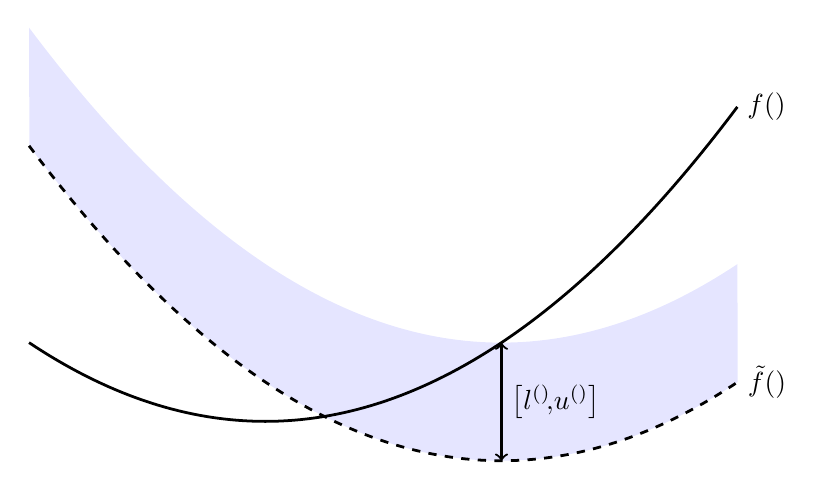
\begin{tikzpicture}[x=3cm, y=1cm]
 % Filled band around the quadratic curve with different boundary curves
\fill[blue!10] 
(-1, 5) -- plot[domain=-2:1, samples=100] ({\x+1}, {\x*\x + 1}) -- 
plot[domain=1:-2, samples=100] ({\x+1}, {\x*\x - 0.5}) -- cycle;
 \node[anchor=west] at (2, 4) {$f(\weights)$};
 \draw[line width=1, domain=-2:1, samples=100,dashed] plot  ({\x+1}, {\x*\x -0.5}) node[right] {$\tilde{f}(\weights)$};
  \draw[line width=1, domain=-1:2, samples=100] plot ({\x}, {\x*\x});
 \draw[<->, thick] (1, -0.5) -- (1, 1) node[midway, right] {$\big[ l^{(\weights)}\!,\!u^{(\weights)} \big]$};
\end{tikzpicture}
\caption{Los métodos de \gls{ml} aprenden \gls{modelparams} $\weights$ usando una estimación de $f(\weights)$ como 
	aproximación del criterio de desempeño $\bar{f}(\weights)$. Usando un \gls{probmodel}, se pueden construir intervalos de confianza $\big[ l^{(\weights)},  u^{(\weights)} \big]$ 
	que contienen $\bar{f}(\weights)$ con alta probabilidad. La mejor medida plausible del desempeño para una elección especifica $\weights$ es $\tilde{f}(\weights) \defeq l^{(\weights)}$.} 
	\end{center}
		\end{figure}},first={optimismo ante la incertidumbre},text={optimismo ante la incertidumbre} 
}

\newglossaryentry{empgraph}
{name={federated learning network (FL network)},
	description={A federated network\index{federated learning network (FL network)} is an undirected weighted \gls{graph} whose 
		nodes represent \gls{data} generators that aim to train a local (or personalized) \gls{model}. 
		Each node in a federated network represents some \gls{device} capable of collecting a \gls{localdataset} 
		and, in turn, train a \gls{localmodel}. 
	    \Gls{fl} methods learn a local \gls{hypothesis} $\localhypothesis{\nodeidx}$, for 
	    each node $\nodeidx \in \nodes$, such that it incurs small \gls{loss} on the \gls{localdataset}s.},first={federated learning network (FL network)},text={FL network} 
}

\newglossaryentry{norm}
{name={norm},
	description={A norm\index{norm} is a function that maps each (vector) element 
		of a linear vector space to a non-negative real number. This function must be homogeneous and definite, and it must satisfy the triangle inequality \cite{HornMatAnalysis}. },
	first={norm},text={norm} 
}

\newglossaryentry{explanation}
{name={explanation},
	description={One approach to make \gls{ml} methods transparent is to provide an 
		explanation\index{explanation} along with the \gls{prediction} delivered by an 
		\gls{ml} method. Explanations can take on many different forms. An explanation 
		could be some natural text or some quantitative measure for the importance 
		of individual \gls{feature}s of a \gls{datapoint} \cite{Molnar2019}. We can also 
		use visual forms of explanations, such as intensity plots for image \gls{classification} \cite{GradCamPaper}.},
	first={explanation},text={explanation} 
}

\newglossaryentry{risk}
{name={risk},
	description={Consider\index{risk} a \gls{hypothesis} $\hypothesis$ used to predict the \gls{label} 
		$\truelabel$ of a \gls{datapoint} based on its \gls{feature}s $\featurevec$. We measure 
		the quality of a particular \gls{prediction} using a \gls{lossfunc} $\lossfunc{(\featurevec,\truelabel)}{\hypothesis}$. 
		If we interpret \gls{datapoint}s as the \gls{realization}s of \gls{iid} \gls{rv}s, 
		also the $\lossfunc{(\featurevec,\truelabel)}{\hypothesis}$ becomes the \gls{realization} 
		of an \gls{rv}. The \gls{iidasspt} allows us to define the risk of a \gls{hypothesis} 
		as the expected \gls{loss} $\expect \big\{\lossfunc{(\featurevec,\truelabel)}{\hypothesis} \big\}$. 
		Note that the risk of $\hypothesis$ depends on both the specific choice for the \gls{lossfunc} and the 
		\gls{probdist} of the \gls{datapoint}s.},
	first={risk},text={risk} 
}

\newglossaryentry{actfun}
{name={activation function},
	description={Each\index{activation function} artificial neuron within an \gls{ann} is 
		assigned an activation function $\actfun(\cdot)$ that maps a weighted combination of 
		the neuron inputs $\feature_{1},\ldots,\feature_{\nrfeatures}$ to a single output 
		value $a = \actfun\big(\weight_{1} \feature_{1}+\ldots+\weight_{\nrfeatures} \feature_{\nrfeatures} \big)$. 
		Note that each neuron is parametrized by the \gls{weights} $\weight_{1},\ldots,\weight_{\nrfeatures}$.},
first={activation function},text={activation function} 
}

\newglossaryentry{distributedalgorithm}
{name={distributed algorithm},
	description={A\index{distributed algorithm} distributed \gls{algorithm} is an \gls{algorithm} designed for 
		a special type of computer: a collection of interconnected computing devices (or nodes). 
		These devices communicate and coordinate their local computations by exchanging 
		messages over a network \cite{IntroDistAlg,ParallelDistrBook}. Unlike a classical \gls{algorithm}, 
		which is implemented on a single \gls{device}, a distributed \gls{algorithm} is 
		executed concurrently on multiple \gls{device}s with computational capabilities. 
		Similar to a classical \gls{algorithm}, a distributed \gls{algorithm} can be modeled as a 
		set of potential executions. However, each execution in the distributed setting involves 
		both local computations and message-passing events. A generic execution might look as 
		follows:
		\[
		\begin{array}{l}
			\text{Node 1: } {\rm input}_1, s_1^{(1)}, s_2^{(1)}, \ldots, s_{T_1}^{(1)}, {\rm output}_1; \\
			\text{Node 2: } {\rm input}_2, s_1^{(2)}, s_2^{(2)}, \ldots, s_{T_2}^{(2)}, {\rm output}_2; \\
			\quad \vdots \\
			\text{Node N: } {\rm input}_N, s_1^{(N)}, s_2^{(N)}, \ldots, s_{T_N}^{(N)}, {\rm output}_N.
		\end{array}
		\]
		Each \gls{device} $\nodeidx$ starts from its own local input and performs a sequence of 
		intermediate computations $s_{\iteridx}^{(\nodeidx)}$ at discrete time instants $\iteridx = 1, \dots, T_\nodeidx$. 
		These computations may depend on both: the previous local computations at the \gls{device} 
		and messages received from other \gls{device}s. One important application of distributed 
		\gls{algorithm}s is in \gls{fl} where a network of \gls{device}s collaboratively train a personal \gls{model} 
		for each \gls{device}. 
		},
	first={distributed algorithm}, text={distributed algorithm}
}


\newglossaryentry{algorithm}
{name={algorithm},
  description={An\index{algorithm} algorithm is a precise, step-by-step specification for 
  	how to produce an output from a given input within a finite number of computational steps \cite{Cormen:2022aa}. 
    For example, an algorithm for training a \gls{linmodel} explicitly describes how to 
	transform a given \gls{trainset} into \gls{modelparams} through a sequence of \gls{gradstep}s. 
    This informal characterization can be formalized rigorously via different mathematical \gls{model}s \cite{Sipser2013}. 
    One very simple \gls{model} of an algorithm is a collection of possible executions. Each execution is a sequence:
    $${\rm input},s_1,s_2,\ldots,s_T,{\rm output}$$ 
    that respects the constraints inherent to the computer executing the algorithm.
	Algorithms may be deterministic, where each input results uniquely in a single execution,
	or randomized, where executions can vary probabilistically. Randomized algorithms 
	can thus be analyzed by modeling execution sequences as outcomes of random experiments, 
	viewing the algorithm as a stochastic process \cite{RandomizedAlgos,BertsekasProb,Gallager13}.
	Crucially, an algorithm encompasses more than just a mapping from input to output; it also includes 
	the intermediate computational steps $s_1,\ldots,s_T$. 
	%. In \textbf{online algorithms}, these intermediate computational steps  can dynamically incorporate additional input data as the execution progresses.
	},
	first={algorithm},text={algorithm} 
}

\newglossaryentry{onlinealgorithm}
{name={online algorithm},
	description={An\index{online algorithm} online \gls{algorithm} processes input \gls{data} incrementally, 
		receiving \gls{data} items sequentially and making decisions or producing outputs (or decisions) immediately 
		without having access to the entire input in advance \cite{HazanOCO,PredictionLearningGames}. 
		Unlike an offline \gls{algorithm}, which has the entire input available from the start, an online \gls{algorithm} 
		must handle uncertainty about future inputs and cannot revise past decisions. Similar to an 
		offline \gls{algorithm}, an online \gls{algorithm} can be modeled formally as a collection of possible 
		executions. However, the execution sequence for an online \gls{algorithm} has a distinct structure:
		$${\rm init},s_1,{\rm out}_{1},{\rm in}_{2},s_2,{\rm out}_{2},\ldots,{\rm in}_{T},s_T,{\rm out}_{T}.$$ 
		Each execution begins from an initial state (\(\text{init}\)) and proceeds through alternating computational steps, 
		outputs (or decisions), and inputs. Specifically, at step \(\iteridx\), the \gls{algorithm} performs a computational step 
		\(s_{\iteridx}\), generates an output \(\text{out}_{\iteridx}\), and then subsequently 
		receives the next input \(\text{in}_{\iteridx+1}\). A notable example of an online \gls{algorithm} in \gls{ml} is 
		\gls{onlineGD} (online gradient descent), which incrementally updates \gls{modelparams} as new \gls{datapoint}s 
		arrive.
	},
	first={online algorithm},text={online algorithm} 
}



%\newglossaryentry{transparency}
%{name={transparency},
%	description={Transparency\index{transparency} is a key requirement for 
%		trustworthy \gls{ai} \cite{HLEGTrustworhtyAI}. In the context of ML methods, 
%		such as \gls{erm}-based methods, transparency is mainly used synonymously 
%		for \gls{explainability} \cite{gallese2023ai,JunXML2020}. However, in the wide 
%		context of \gls{ai} systems, transparency also includes providing information 
%		about limitations and reliability of the \gls{ai} system. As a point in case, \gls{logreg} provides a 
%		quantitative measure of the reliability of a \gls{classification} in the form of the value $|\hypothesis(\featurevec)|$. 
%		Transparency also includes the user interface, by requiring to clearly indicate when a user is 
%		interaction with an \gls{ai} system. Another component of transparency is the documentation 
%		of the system’s purpose, design choices, and intended use cases \cite{Shahriari2017,DatasheetData2021,10.1145/3287560.3287596}. },
%	first={transparency},text={transparency} 
%}

\newglossaryentry{transparency}
{name={transparency},
	description={Transparency\index{transparency} is a fundamental requirement for 
		\gls{trustAI} \cite{HLEGTrustworhtyAI}. In the context of \gls{ml} 
		methods, transparency is often used interchangeably with \gls{explainability} 
		\cite{gallese2023ai,JunXML2020}. However, in the broader scope of \gls{ai} 
		systems, transparency extends beyond \gls{explainability} and includes providing information 
		about the system’s limitations, reliability, and intended use. 
		In medical diagnosis systems, transparency requires disclosing the confidence level 
		for the \gls{prediction}s delivered by a trained \gls{model}. In credit scoring, 
		\gls{ai}-based lending decisions should be accompanied by explanations of 
		contributing factors, such as income level or credit history. These explanations 
		allow humans (e.g., a loan applicant) to understand and contest automated decisions. 
		Some \gls{ml} methods inherently offer transparency. For example, \gls{logreg} 
		provides a quantitative measure of \gls{classification} reliability through the value $|\hypothesis(\featurevec)|$. 
		\Gls{decisiontree}s are another example, as they allow human-readable decision rules \cite{rudin2019stop}.
		Transparency also requires a clear indication when a user is engaging with an \gls{ai} system. 
		For example, \gls{ai}-powered chatbots should notify users that they are interacting with an 
		automated system rather than a human. Furthermore, transparency encompasses comprehensive 
		documentation detailing the purpose and design choices underlying the \gls{ai} system. 
		For instance, \gls{model} datasheets \cite{DatasheetData2021} and \gls{ai} system cards \cite{10.1145/3287560.3287596} 
		help practitioners understand the intended use cases and limitations of an \gls{ai} system \cite{Shahriari2017}.},
	first={transparency}, text={transparency} 
}



\newglossaryentry{sensattr}
{name={sensitive attribute},
	description={\gls{ml}\index{sensitive attribute} revolves around learning a \gls{hypothesis} map that allows 
		us to predict the \gls{label} of a \gls{datapoint} from its \gls{feature}s. In some 
		applications, we must ensure that the output delivered by an \gls{ml} system does 
		not allow us to infer sensitive attributes of a \gls{datapoint}. Which part 
		of a \gls{datapoint} is considered a sensitive attribute is a design 
		choice that varies across different application domains.},
	first={sensitive attribute},text={sensitive attribute} 
}


\newglossaryentry{sbm}
{name={stochastic block model (SBM)},
	description={The\index{stochastic block model (SBM)} stochastic block \gls{model} is a 
		probabilistic generative \gls{model} for an undirected \gls{graph} $\graph = \big( \nodes, \edges \big)$ 
		with a given set of nodes $\nodes$ \cite{AbbeSBM2018}. In its most basic variant, 
		the stochastic block \gls{model} generates a \gls{graph} by first randomly assigning each node $\nodeidx \in \nodes$ to 
		a \gls{cluster} index $\clusteridx_{\nodeidx} \in \{1,\ldots,\nrcluster\}$. A pair of different nodes in the 
		\gls{graph} is connected by an edge with \gls{probability} $p_{\nodeidx,\nodeidx'}$ that depends 
		solely on the \gls{label}s $\clusteridx_{\nodeidx}, \clusteridx_{\nodeidx'}$. 
		The presence of edges between different pairs of 
		nodes is statistically independent. },
	first={stochastic block model (SBM)},text={SBM} 
}

\newglossaryentry{deepnet}
{name={deep net},
	description={A\index{deep net} deep net is an \gls{ann} with a (relatively) large number of 
	hidden layers. Deep learning is an umbrella term for \gls{ml} methods that use a deep 
	net as their \gls{model} \cite{Goodfellow-et-al-2016}.},
	first={deep net},text={deep net} 
}

\newcommand{\gaussiancenter}{3}

\newglossaryentry{baseline}
{name={baseline},
    description={Consider\index{baseline} some \gls{ml} method that produces a learned 
    	\gls{hypothesis} (or trained \gls{model}) $\learnthypothesis \in \hypospace$. We evaluate the quality of a trained \gls{model} 
    by computing the average \gls{loss} on a \gls{testset}. But how can we assess 
    whether the resulting \gls{testset} performance is sufficiently good? How can we 
    determine if the trained \gls{model} performs close to optimal and there is little point 
    in investing more resources (for \gls{data} collection or computation) to improve it? 
    To this end, it is useful to have a reference (or baseline) level against which 
    we can compare the performance of the trained \gls{model}. Such a reference value 
    might be obtained from human performance, e.g., the misclassification rate of dermatologists 
    who diagnose cancer from visual inspection of skin \cite{SkinHumanAI}. Another source for a baseline is an existing, 
    but for some reason unsuitable, \gls{ml} method. For example, the existing \gls{ml} method 
    might be computationally too expensive for the intended \gls{ml} application. 
    Nevertheless, its \gls{testset} error can still serve as a baseline. Another, somewhat more principled, 
    approach to constructing a baseline is via a \gls{probmodel}. In many cases, given a \gls{probmodel} $p(\featurevec,\truelabel)$,  
    we can precisely determine the \gls{minimum} achievable \gls{risk} among any hypotheses
    (not even required to belong to the \gls{hypospace} $\hypospace$) \cite{LC}. 
    This \gls{minimum} achievable \gls{risk} (referred to as the \gls{bayesrisk}) is the \gls{risk} 
    of the \gls{bayesestimator} for the \gls{label} $\truelabel$ of a \gls{datapoint}, given
    its \gls{feature}s $\featurevec$. Note that, for a given choice of \gls{lossfunc}, the 
    \gls{bayesestimator} (if it exists) is completely determined by the \gls{probdist} $p(\featurevec,\truelabel)$ \cite[Ch. 4]{LC}. 
    However, computing the \gls{bayesestimator} and \gls{bayesrisk} presents two 
    main challenges:
    \begin{enumerate}[label=\arabic*)]
    	\item The \gls{probdist} $p(\featurevec,\truelabel)$ is unknown and 
    needs to be estimated.
    	\item Even if $p(\featurevec,\truelabel)$ is known, 
    it can be computationally too expensive to compute the \gls{bayesrisk} exactly \cite{cooper1990computational}. 
   \end{enumerate}
A widely used \gls{probmodel} is the \gls{mvndist} $\pair{\featurevec}{\truelabel} \sim \mathcal{N}({\bm \mu},{\bm \Sigma})$ 
for \gls{datapoint}s characterized by numeric \gls{feature}s and \gls{label}s.
Here, for the \gls{sqerrloss}, the \gls{bayesestimator} is given by the posterior 
\gls{mean} $\mu_{\truelabel|\featurevec}$ of the \gls{label} $\truelabel$, given the 
\gls{feature}s $\featurevec$ \cite{LC,GrayProbBook}. The corresponding \gls{bayesrisk} 
is given by the posterior \gls{variance} 
$\sigma^{2}_{\truelabel|\featurevec}$ (see Figure \ref{fig_post_baseline_dict}).
	\begin{figure}[H]
		\begin{center}
		\begin{tikzpicture}
			% Axes
			\draw[->] (-1,0) -- (7,0) node[right] {$\truelabel$}; % x-axis
			% Gaussian distribution centered at \gaussiancenter with variance 1
			\draw[thick,domain=-1:7,smooth,variable=\x] 
			  plot ({\x}, {2*exp(-0.5*((\x-\gaussiancenter)^2))});
			% Dashed line indicating the mean of the Gaussian
			\draw[dashed] (\gaussiancenter,0) -- (\gaussiancenter,2.5);
			\node[anchor=south] at ([yshift=-5pt] \gaussiancenter,2.5) {\small $\mu_{\truelabel|\featurevec}$};
			% Double arrow indicating the variance
			\draw[<->,thick] (\gaussiancenter-1,1) -- (\gaussiancenter+1,1.0);
			\node[anchor=west] at ([yshift=2pt] \gaussiancenter,1.2) {\small $\sigma_{\truelabel|\featurevec}$};
			% Posterior variance label
			%\node[anchor=south east] at (\gaussiancenter-0.5,1.8) {\small Posterior Variance};
			% x-axis marks with crosses
			  % x-axis marks with crosses
  			\foreach \x in {0.5} {
				\node[red] at (\x, 0) {\bf \large $\times$};
 			 }
  % h(x) label for the first cross
  			\node[anchor=north] at (0.5,-0.2) {\small $\learnthypothesis(\featurevec)$};
		  \end{tikzpicture}
		\end{center}
		\caption{If the \gls{feature}s and the \gls{label} of a \gls{datapoint} are drawn from a \gls{mvndist}, we 
		can achieve the \gls{minimum} \gls{risk} (under \gls{sqerrloss}) by using the \gls{bayesestimator} $\mu_{\truelabel|\featurevec}$ 
		to predict the \gls{label} $\truelabel$ of a \gls{datapoint} with \gls{feature}s $\featurevec$. The corresponding 
		\gls{minimum} \gls{risk} is given by the posterior \gls{variance} $\sigma^{2}_{\truelabel|\featurevec}$. We can use 
		this quantity as a baseline for the average \gls{loss} of a trained \gls{model} $\learnthypothesis$. \label{fig_post_baseline_dict}}
	\end{figure}},
    first={baseline},text={baseline}
}

\newglossaryentry{spectrogram}
{name={spectrogram},
	description={
		A\index{spectrogram} spectrogram represents the time-frequency distribution of the energy of a time signal $x(t)$.  
		Intuitively, it quantifies the amount of signal energy present within a specific time segment 
		$[t_{1},t_{2}] \subseteq \mathbb{R}$ and frequency interval $[f_{1},f_{2}]\subseteq \mathbb{R}$. 
		Formally, the spectrogram of a signal is defined as the squared magnitude of its 
		short-time Fourier transform (STFT) \cite{cohen1995time}.
        Figure \ref{fig:spectrogram_dict} depicts a time signal along with its spectrogram. 
	\begin{figure}[H]
		\centering
		\includegraphics[width=0.8\textwidth]{assets/spectrogram.png}
		\caption{Left: A time signal consisting of two modulated Gaussian pulses. Right: An intensity 
		plot of the spectrogram.
		\label{fig:spectrogram_dict}}
	\end{figure}
        The intensity plot of its spectrogram can serve as an image of a signal. A 
		simple recipe for audio signal \gls{classification} is to feed this signal image 
		into \gls{deepnet}s originally developed for image \gls{classification} and object detection \cite{Li:2022aa}. 
		It is worth noting that, beyond the spectrogram, several alternative representations exist 
		for the time-frequency distribution of signal energy \cite{TimeFrequencyAnalysisBoashash,MallatBook}. 
		}, 
	first={spectrogram},text={spectrogram} 
}

\newglossaryentry{graphclustering}
{name={graph clustering},
	description={\Gls{graph} \gls{clustering}\index{graph clustering} aims at 
		\gls{clustering} \gls{datapoint}s that are represented as the nodes 
		of a \gls{graph} $\graph$. The edges of $\graph$ represent 
		pairwise similarities between \gls{datapoint}s. Sometimes we
		can quantify the extend of these similarities by an \gls{edgeweight} \cite{Luxburg2007,FlowSpecClustering2021}. }, 
	first={graph clustering},text={graph clustering} 
}

\newglossaryentry{specclustering}
{name={spectral clustering},
	description={Spectral \gls{clustering}\index{spectral clustering} is a particular instance of 
		\gls{graphclustering}, i.e., it clusters \gls{datapoint}s 
		represented as the nodes $\nodeidx=1,\ldots,\nrnodes$ of a \gls{graph} $\graph$. 
		Spectral \gls{clustering} uses the \gls{eigenvector}s of the \gls{LapMat} $\LapMat{\graph}$ 
		to construct \gls{featurevec}s $\featurevec^{(\nodeidx)} \in \mathbb{R}^{\nrfeatures}$ 
		for each node (i.e., for each \gls{datapoint}) $\nodeidx=1,\ldots,\nrnodes$. We can feed these \gls{featurevec}s 
		into \gls{euclidspace}-based \gls{clustering} methods, such as \gls{kmeans} 
		or \gls{softclustering} via \gls{gmm}. Roughly speaking, the \gls{featurevec}s of nodes 
		belonging to a well-connected subset (or \gls{cluster}) of nodes in $\graph$ are located 
		nearby in the \gls{euclidspace} $\mathbb{R}^{\nrfeatures}$ (see Figure \ref{fig_lap_mtx_specclustering_dict}). 
		\begin{figure}[H]
			\begin{center}
				\begin{minipage}{0.4\textwidth}
			\begin{tikzpicture}
				% Define the style for filled nodes
				\begin{scope}[every node/.style={circle, fill=black, inner sep=0pt, minimum size=0.3cm}]
					% Define nodes
					\node (1) at (0,0) {};
					\node (2) [below left=of 1, xshift=-0.2cm, yshift=-1cm] {};
					\node (3) [below right=of 1, xshift=0.2cm, yshift=-1cm] {};
					\node (4) [below=of 1, yshift=0.5cm] {}; % Isolated node
				\end{scope}
				% Draw edges
				\draw (1) -- (2);
				\draw (1) -- (3);
				% Add labels (separate from filled nodes)
				\node[above=0.2cm] at (1) {$\nodeidx=1$};
				\node[left=0.3cm] at (2) {$2$};
				\node[right=0.3cm] at (3) {$3$};
				\node[below=0.2cm] at (4) {$4$};
			\end{tikzpicture}
				\end{minipage} 
				\hspace*{5mm}
				\begin{minipage}{0.4\textwidth}
					\begin{equation} 
						\LapMat{\graph}\!=\!
						\begin{pmatrix} 
							2 & -1 & -1 & 0 \\ 
							-1 & 1 & 0 & 0 \\  
							-1 & 0 & 1 & 0 \\ 
							0 & 0 & 0 & 0 
						\end{pmatrix}\!=\!\mathbf{V} {\bm \Lambda} \mathbf{V}^{T}  
						\nonumber
					\end{equation} 
				\end{minipage}
				\vspace*{20mm}\\
				  \begin{minipage}{0.4\textwidth}
				\begin{tikzpicture}[scale=3]
%					% Axes
					\draw[->] (-0.2, 0) -- (1.2, 0) node[right] {$v^{(1)}_{\nodeidx}$};
					\draw[->] (0, -0.2) -- (0, 1.2) node[above] {$v^{(2)}_{\nodeidx}$};
%					
%					% Tailored tick marks and labels
%					\draw (0,0) node[below left] {$0$};
%					\draw (1/sqrt(3), 0) node[below] {$\frac{1}{\sqrt{3}}$} -- ++(0,0.05);
%					\draw (0, 1) node[left] {$1$} -- ++(0.05,0);
%					
%					 Data points
					\filldraw[blue] (0.577, 0) circle (0.03cm) node[above right] {$\nodeidx=1,2,3$};
					\filldraw[blue] (0.577, 0) circle (0.03cm); % Second point overlaps
					\filldraw[blue] (0.577, 0) circle (0.03cm); % Third point overlaps
					\filldraw[red] (0, 1) circle (0.03cm) node[above right] {$4$};
%					% Grid for reference
%					\draw[dashed, gray] (1/sqrt(3), 0) -- (1/sqrt(3), 1);
%					\draw[dashed, gray] (0, 1) -- (1, 1);
				\end{tikzpicture}
				\end{minipage} 
    		\begin{minipage}{0.4\textwidth}
										\begin{align}
											& \mathbf{V} = \big( \vv^{(1)},\vv^{(2)},\vv^{(3)},\vv^{(4)} \big) \nonumber \\
											&	\mathbf{v}^{(1)}\!=\!\frac{1}{\sqrt{3}} \begin{pmatrix} 1 \\ 1 \\ 1 \\ 0 \end{pmatrix}, \,
												\mathbf{v}^{(2)}\!=\!\begin{pmatrix} 0 \\ 0 \\ 0 \\ 1 \end{pmatrix} \nonumber 
												\end{align}
				\end{minipage} 
				\caption{\label{fig_lap_mtx_specclustering_dict} {\bf Top.} Left: An undirected \gls{graph} 
					$\graph$ with four nodes $\nodeidx=1,2,3,4$, each representing a \gls{datapoint}. Right: The \gls{LapMat} 
					$\LapMat{\graph}  \in \mathbb{R}^{4 \times 4}$ and its \gls{evd}. 
					{\bf Bottom.} Left: A \gls{scatterplot} of \gls{datapoint}s using the \gls{featurevec}s 
					$\featurevec^{(\nodeidx)} = \big( v^{(1)}_{\nodeidx},v^{(2)}_{\nodeidx} \big)^{T}$. 
					Right: Two \gls{eigenvector}s $\vv^{(1)},\vv^{(2)} \in \mathbb{R}^{\nrfeatures}$ 
					corresponding to the \gls{eigenvalue} $\lambda=0$ of the \gls{LapMat} $\LapMat{\graph}$. 
					} 
			\end{center}
		\end{figure}
	\newpage}, 
	first={spectral clustering},text={spectral clustering} 
}

\newglossaryentry{flowbasedclustering}
{name={flow-based clustering},
	description={Flow-based \gls{clustering}\index{flow-based clustering} groups the nodes 
		of an undirected \gls{graph} by applying \gls{kmeans} \gls{clustering} to node-wise 
		\gls{featurevec}s. These \gls{featurevec}s are built from network flows between 
		carefully selected sources and destination nodes \cite{FlowSpecClustering2021}. }, 
	first={flow-based clustering},text={flow-based clustering} 
}



\newglossaryentry{esterr}
{name={estimation error},
	description={Consider\index{estimation error} \gls{datapoint}s, each with \gls{featurevec} $\featurevec$ and \gls{label} 
		$\truelabel$. In some applications, we can model the relation between the \gls{featurevec} and the \gls{label}
		of a \gls{datapoint} as $\truelabel = \bar{\hypothesis}(\featurevec) + \varepsilon$. Here, we 
		use some true underlying \gls{hypothesis} $\bar{\hypothesis}$ and a noise term $\varepsilon$ 
		which summarizes any modeling or labeling errors. The estimation error incurred by an \gls{ml} 
		method that learns a \gls{hypothesis} $\widehat{\hypothesis}$, e.g., using \gls{erm}, is defined as 
		$\widehat{\hypothesis}(\featurevec) - \bar{\hypothesis}(\featurevec)$, for some \gls{featurevec}. 
		For a parametric \gls{hypospace}, which consists of \gls{hypothesis} maps determined by 
		\gls{modelparams} $\weights$, we can define the estimation error as $\Delta \weights = \widehat{\weights} - \overline{\weights}$ \cite{kay,hastie01statisticallearning}.},
	first={estimation error},text={estimation error} 
}


\newglossaryentry{dob}
{name={degree of belonging},
	description={Degree of belonging\index{degree of belonging} is a number that indicates the extent to which a \gls{datapoint} 
		belongs to a \gls{cluster} \cite[Ch. 8]{MLBasics}. The degree of belonging can be 
		interpreted as a soft \gls{cluster} assignment. \Gls{softclustering} methods can 
		encode the degree of belonging by a real number in the interval $[0,1]$. 
		\Gls{hardclustering} is obtained as the extreme case when the degree of belonging 
		only takes on values $0$ or $1$.}, first={degree of belonging},text={degree of belonging} 
}

\newglossaryentry{msee}
{name={mean squared estimation error (MSEE)},
	description={Consider\index{mean squared estimation error (MSEE)} an \gls{ml} method that 
		learns \gls{modelparams} $\widehat{\weights}$ based on some \gls{dataset} $\dataset$. 
		If we interpret the \gls{datapoint}s in $\dataset$ as \gls{iid} \gls{realization}s of an \gls{rv} $\datapoint$, 
		we define the \gls{esterr} $\Delta \weights \defeq \widehat{\weight} - \overline{\weights}$. 
		Here, $\overline{\weights}$ denotes the true \gls{modelparams} of the \gls{probdist} 
		of $\datapoint$. The \gls{mean} squared \gls{esterr} is 
		defined as the \gls{expectation} $\expect \big\{ \big\| \Delta \weights \big\|^{2} \big\}$ of the 
		squared Euclidean \gls{norm} of the \gls{esterr} \cite{LC,kay}.},
	first={mean squared estimation error (MSEE)},text={MSEE} 
}

\newglossaryentry{gtvmin}
{name={generalized total variation minimization (GTVMin)},
	description={\gls{gtv} minimization\index{generalized total variation minimization (GTVMin)} is an instance of \gls{rerm} 
		using the \gls{gtv} of local \gls{modelparams} as a \gls{regularizer} \cite{ClusteredFLTVMinTSP}.},
	first={generalized total variation minimization (GTVMin)},text={GTVMin} 
}

\newglossaryentry{regression}
{name={regression},
	description={Regression\index{regression} problems revolve around the 
		prediction of a numeric \gls{label} solely from the \gls{feature}s of a \gls{datapoint} \cite[Ch. 2]{MLBasics}.},
	first={regression},text={regression} 
}

\newglossaryentry{acc}
{name={accuracy},
	description={Consider\index{accuracy} \gls{datapoint}s characterized by \gls{feature}s $\featurevec \in \featurespace$ and 
		a categorical label $\truelabel$ which takes on values from a finite \gls{labelspace} $\labelspace$. The 
		accuracy of a \gls{hypothesis} $\hypothesis: \featurespace \rightarrow \labelspace$, when applied 
		to the \gls{datapoint}s in a \gls{dataset} $\dataset = \big\{ \big(\featurevec^{(1)}, \truelabel^{(1)} \big), \ldots, \big(\featurevec^{(\samplesize)},\truelabel^{(\samplesize)}\big) \big\}$, 
		is then defined as $1 - (1/\samplesize)\sum_{\sampleidx=1}^{\samplesize} \lossfunczo{\big(\featurevec^{(\sampleidx)},\truelabel^{(\sampleidx)}\big)}{\hypothesis}$ using the \gls{zerooneloss} $\lossfunczo{\cdot}{\cdot}$.},
	first={accuracy},text={accuracy} 
}





\newglossaryentry{expert}
{name={expert},
	description={\gls{ml}\index{expert} aims to learn a \gls{hypothesis} $\hypothesis$ that accurately predicts the \gls{label} 
		of a \gls{datapoint} based on its \gls{feature}s. We measure the \gls{prediction} error using 
		some \gls{lossfunc}. Ideally, we want to find a \gls{hypothesis} that incurs minimal \gls{loss} 
		on any \gls{datapoint}. We can make this informal goal precise via the \gls{iidasspt} 
		and by using the \gls{bayesrisk} as the \gls{baseline} for the (average) \gls{loss} of a \gls{hypothesis}. 
		An alternative approach to obtaining a \gls{baseline} is to use the \gls{hypothesis} $\hypothesis'$ learned 
		by an existing \gls{ml} method. We refer to this \gls{hypothesis} $\hypothesis'$ as an expert \cite{PredictionLearningGames}. \Gls{regret} minimization methods learn a \gls{hypothesis}
		that incurs a \gls{loss} comparable to the best expert \cite{PredictionLearningGames,HazanOCO}.},
	first={expert},text={expert} 
}

\newglossaryentry{nfl}
{name={networked federated learning (NFL)},
	description={Networked \gls{fl}\index{networked federated learning (NFL)} refers 
		to methods that learn personalized \gls{model}s in a distributed fashion. These methods learn from \gls{localdataset}s 
		that are related by an intrinsic network structure.},
 first={networked federated learning (NFL)},text={NFL} 
}




\newglossaryentry{regret}
{name={regret},
	description={The regret\index{regret} of a \gls{hypothesis} $\hypothesis$ relative to 
		another \gls{hypothesis} $\hypothesis'$, which serves as a \gls{baseline}, 
		is the difference between the \gls{loss} incurred by $\hypothesis$ and the \gls{loss} 
		incurred by $\hypothesis'$ \cite{PredictionLearningGames}. 
		The \gls{baseline} \gls{hypothesis} $\hypothesis'$ is also referred to as an \gls{expert}.},
	first={regret},text={regret} 
}

\newglossaryentry{strcvx}
{name={strongly convex},
	description={A\index{strongly convex} continuously \gls{differentiable} real-valued 
		function $f(\featurevec)$ is strongly \gls{convex} with coefficient $\sigma$ if $f(\vy) \geq f(\vx) + \nabla f(\vx)^{T} (\vy - \vx) + (\sigma/2) \normgeneric{\vy - \vx}{2}^{2}$ \cite{nesterov04},\cite[Sec. B.1.1]{CvxAlgBertsekas}.},
	first={strongly convex},text={strongly convex} 
}

\newglossaryentry{differentiable}
{name={differentiable},
	description={A\index{differentiable} real-valued function $f: \mathbb{R}^{\featuredim} \rightarrow \mathbb{R}$ 
		is differentiable if it can, at any point, be approximated locally by a linear 
		function. The local linear approximation at the point $\mathbf{x}$ is determined 
		by the \gls{gradient} $\nabla f ( \mathbf{x})$ \cite{RudinBookPrinciplesMatheAnalysis}.},
	first={differentiable},text={differentiable} 
}

\newglossaryentry{gradient}
{name={gradient},
	description={For\index{gradient} a real-valued function $f: \mathbb{R}^{\featuredim} \rightarrow \mathbb{R}: \weights \mapsto f(\weights)$, 
	a vector $\vg$ such that $\lim_{\weights \rightarrow \weights'} \frac{f(\weights) - \big(f(\weights')+ \vg^{T} (\weights- \weights') \big) }{\| \weights-\weights'\|}=0$ 
	is referred to as the gradient of $f$ at $\weights'$. If such a vector exists, it is 
	denoted $\nabla f(\weights')$ or $\nabla f(\weights)\big|_{\weights'}$ \cite{RudinBookPrinciplesMatheAnalysis}.},
	first={gradient},text={gradient} 
}

\newglossaryentry{subgradient}
{name={subgradient},
description={For\index{subgradient} a real-valued function $f: \mathbb{R}^{\featuredim} \rightarrow \mathbb{R}: \weights \mapsto f(\weights)$, 
		a vector $\va$ such that $f(\weights) \geq  f(\weights') +\big(\weights-\weights' \big)^{T} \va$ is 
		referred to as a subgradient of $f$ at $\weights'$ \cite{BertCvxAnalOpt,BertsekasNonLinProgr}.},
	first={subgradient},text={subgradient} 
}

\newglossaryentry{fedavg}
{name={federated averaging (FedAvg)},
	description={FedAvg\index{federated averaging (FedAvg)} refers to an iterative \gls{fl} \gls{algorithm} that alternates between separately training \gls{localmodel}s and combining the updated local \gls{modelparams}. The training of \gls{localmodel}s 
		is implemented via several \gls{stochGD} steps \cite{pmlr-v54-mcmahan17a}.}, 
		first = {FedAvg}, text={FedAvg} 
}

\newglossaryentry{fedprox}
{name={FedProx},
	description={FedProx\index{FedProx} refers to an iterative \gls{fl} \gls{algorithm} that alternates between separately training \gls{localmodel}s and combining the updated local \gls{modelparams}. In contrast to \gls{fedavg}, which uses 
		\gls{stochGD} to train \gls{localmodel}s, FedProx uses a \gls{proxop} for the training \cite{FedProx2020}.}, 
	first = {FedProx}, text={FedProx} 
}

\newglossaryentry{relu}
{name={rectified linear unit (ReLU)},
	description={The\index{rectified linear unit (ReLU)} ReLU is 
		a popular choice for the \gls{actfun} of a neuron within an \gls{ann}. It is defined 
		as $\actfun(z) = \max\{0,z\}$, with $z$ being the weighted input of the artificial 
		neuron.}, first = {rectified linear unit (ReLU)}, text={ReLU} 
}

\newglossaryentry{hypothesis}
{name={hypothesis},
	description={A\index{hypothesis} hypothesis refers to a map (or function) $\hypothesis: \featurespace \rightarrow \labelspace$ from the 
		\gls{featurespace} $\featurespace$ to the \gls{labelspace} $\labelspace$. 
		Given a \gls{datapoint} with \gls{feature}s $\featurevec$, we use a hypothesis map $\hypothesis$
		to estimate (or approximate) the \gls{label} $\truelabel$ using the \gls{prediction}  
		$\hat{\truelabel} = \hypothesis(\featurevec)$. \Gls{ml} is all about learning (or finding) a 
		hypothesis map $\hypothesis$ such that $\truelabel \approx \hypothesis(\featurevec)$ 
		for any \gls{datapoint} (having \gls{feature}s $\featurevec$ and \gls{label} $\truelabel$).},
	first={hypothesis},text={hypothesis}  
}



\newglossaryentry{vcdim}
{name={Vapnik–Chervonenkis dimension (VC dimension)},
	description={The\index{Vapnik–Chervonenkis dimension (VC dimension)} VC dimension of an infinite \gls{hypospace} is a widely-used measure 
		for its size. We refer to the literature (see \cite{ShalevMLBook}) for a precise definition of VC dimension 
		as well as a discussion of its basic properties and use in \gls{ml}.},
	first={Vapnik–Chervonenkis dimension (VC dimension)},text={VC dimension}  
}

\newglossaryentry{effdim}
{name={effective dimension},
	description={The\index{effective dimension} effective dimension $\effdim{\hypospace}$ of 
		an infinite \gls{hypospace} $\hypospace$ is a measure of its size. Loosely speaking, the 
		effective dimension is equal to the effective number of independent tunable \gls{modelparams}. 
		These \gls{parameters} might be the coefficients used in a linear map or the 
		\gls{weights} and bias terms of an \gls{ann}.},
	first={effective dimension},text={effective dimension}  
}

\newglossaryentry{labelspace}
{name={label space},
	description={Consider\index{label space} an \gls{ml} application that involves \gls{datapoint}s characterized by \gls{feature}s 
		and \gls{label}s. The \gls{label} space is constituted by all potential values that the \gls{label} 
		of a \gls{datapoint} can take on. \Gls{regression} methods, aiming at predicting numeric \gls{label}s, often
		 use the \gls{label} space $\labelspace = \mathbb{R}$. Binary \gls{classification} methods use a \gls{label} space 
 		that consists of two different elements, e.g., $\labelspace =\{-1,1\}$, $\labelspace=\{0,1\}$, 
		or $\labelspace = \{ \mbox{``cat image''}, \mbox{``no cat image''} \}$.}, first={label space},text={label space}  
}

\newglossaryentry{prediction}
{name={prediction},
	description={A\index{prediction} prediction is an estimate or approximation for some 
		quantity of interest. \Gls{ml} revolves around learning or finding a \gls{hypothesis} map $\hypothesis$ 
		that reads in the \gls{feature}s $\featurevec$ of a \gls{datapoint} and delivers a prediction 
		$\widehat{\truelabel} \defeq \hypothesis(\featurevec)$ for its \gls{label} $\truelabel$. },
	first={prediction},text={prediction}  
}


\newglossaryentry{histogram}
{name={histogram},
	description={Consider\index{histogram} a \gls{dataset} $\dataset$ that consists of $\samplesize$ \gls{datapoint}s 
		$\datapoint^{(1)},\ldots,\datapoint^{(\samplesize)}$, each of them belonging to some 
		cell $[-U,U] \times \ldots \times [-U,U] \subseteq \mathbb{R}^{\featuredim}$ with side 
		length $U$. We partition this cell evenly into smaller elementary cells with side 
		length $\Delta$. The histogram of $\dataset$ assigns each elementary cell to 
		the corresponding fraction of \gls{datapoint}s in $\dataset$ that fall into this 
		elementary cell. 
	},
	first={histogram},text={histogram}  
}
